%--------------------
% CHAPTER 8: Results
%--------------------

\chapter{Results}

\label{chapter08}

How the system keeps running every day? After every day execution a notification is sent to the contact mail (felix.arribas@skyscanner.net). If something goes wring, is easy to find the logs in Amazon Web Services and create a ticket in the related project.
\\\\
Right now the database does not have much data. Is very difficult to extract tendencies, there are only records from the last two months. Even so, there is enough to make some conclusions from the different comparisons.
\\\\
There are some examples of usage of the \thesis.

\subsection*{Experiment 1} \label{exp1}

What London airport people prefer when traveling from Barcelona?
\\\\
There are six airports in London, searching user demand from Barcelona to those airports for traveling in October 2018 we get the following chart:

\begin{figure}[H]
\centering
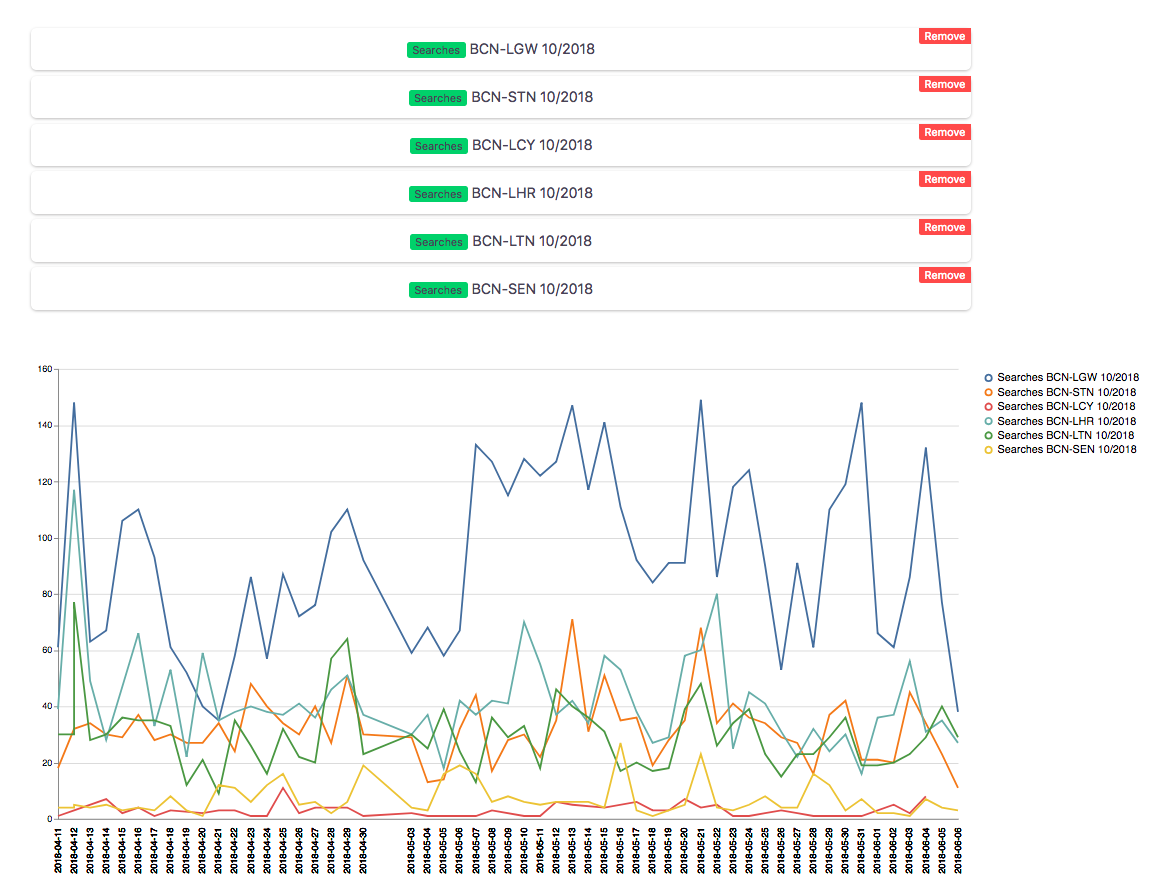
\includegraphics[scale=0.3]{resources/experiment01.png}
\caption{Searches from Barcelona to London Airports October 2018}
\end{figure}

From its six airports: City, Heathrow, Gatwick, Luton, Stansted and Southend; Heathrow is the London Airport with more passengers (78 million in 2017\cite{london_traffic}) but Gatwick (45 million passengers in 2017) is the preferred airport when traveling from Barcelona.

\subsection*{Experiment 2} \label{exp2}

When traveling from New York (JFK), the results are different:

\begin{figure}[H]
\centering
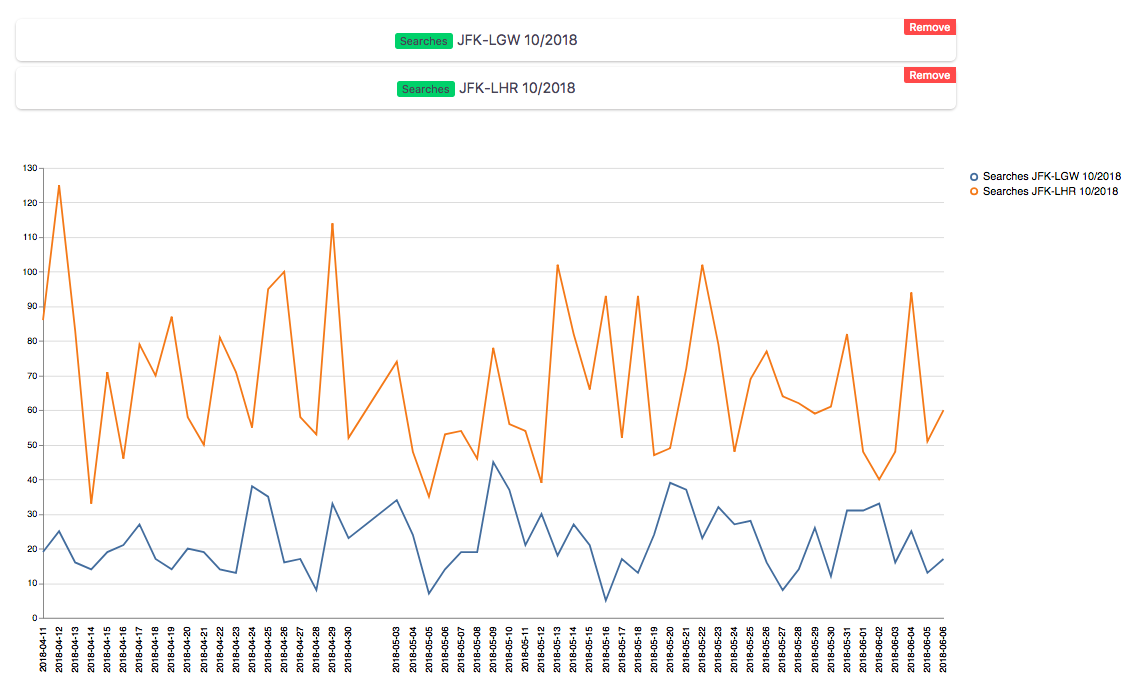
\includegraphics[scale=0.35]{resources/experiment02.png}
\caption{Searches from New York JFK to LHR and LGW October 2018}
\end{figure}

London Heathrow is searched more than London Gatwick. Provably because Heathrow usually operates longer flights than Gatwick airport.
\\\\
